
\chapter{Representation Of Spatial Relations In Neural Language Models}
\chaptersource{Mehdi Ghanimifard and Simon Dobnik.}{\emph{What} a neural language model tells us about spatial relations,}{In Proceedings of the Combined Workshop on Spatial Language Understanding (SpLU) and Grounded Communication for Robotics (RoboNLP), pp. 71-81. 2019.}

\paragraph{Abstract}
Understanding and generating spatial descriptions requires knowledge about
\emph{what} objects are related, their functional interactions, and \emph{where} the objects are geometrically
located. Different spatial relations have different functional and geometric bias. The wide usage of neural language models in different areas including
generation of image description motivates the study of what kind of knowledge
is encoded in neural language models about individual spatial relations. With the premise
that the functional bias of relations is expressed in their word distributions, we construct multi-word
distributional vector representations and show that these representations
perform well on intrinsic semantic reasoning tasks, thus confirming our premise. A comparison of our vector representations to human
semantic judgments indicates that different bias (functional or
geometric) is captured in different data collection tasks which suggests that the contribution of the two meaning modalities is dynamic, related to the context of the task.



\section{Introduction}

Spatial descriptions such as ``the chair is to the left of the table'' contain
spatial relations ``to the left of'' the semantic representations of which must
be grounded in visual representations in terms of geometry
\cite{harnad1990symbol}. The apprehension of spatial relations in terms of
scene geometry has been investigated through acceptability scores of human
judges over possible locations of objects \cite{logan/sadler:1996}. In
addition, other research has pointed out that there is an interplay between
geometry and object-specific function in the apprehension of spatial relations
\cite{coventry2001interplay}.
Therefore, spatial descriptions must be grounded in two kinds of knowledge \cite{Landau:1993aa,coventry2001interplay,Coventry:2004aa,Landau:2016aa}.
One kind of knowledge is referential meaning, expressed in the geometry of
scenes (geometric knowledge or \emph{where} objects are) while the other kind of knowledge is higher-
level conceptual world knowledge about interactions between objects which is
not directly grounded in perceivable situations but is learned through our
experience of situations in the world (functional knowledge or \emph{what} objects are related).
Furthermore, \citet{coventry2001interplay} argue that individual relations have a
particular geometric and functional bias and
``\emph{under}" and ``\emph{over}" are more functionally-biased than ``\emph{below}" and ``\emph{above}". For instance, when describing the relation between a person and an umbrella in a scene with a textual context such as
``$an~umbrella~\underline{\hspace{0.5cm}}~a~person$", ``\emph{above}" is
associated with stricter geometric properties compared to ``\emph{over}" which
covers a more object-specific extra-geometric sense between the target and
the landmark (i.e. \emph{covering} or \emph{protecting} in this case). Of course, there will be several configurations of objects that could be described either with ``\emph{over}" or ``\emph{above}" which indicates that the choice of a description is determined by the speaker, in particular what aspect of meaning they want to emphasise. %
\citet{coventry2001interplay} consider this bias for prepositions that are geometrically similar and therefore the functional knowledge is reflected in different preferences for objects that are related. However, such functional differences also exist between geometrically different relations.


This poses two interesting research questions for computational modelling of
spatial language. The first one is %
how both kinds of
knowledge interact with individual spatial relations and how models of spatial
language can be constructed and learned within end-to-end deep learning
paradigm. \citet{ramisa2015combining} compare the performance of classifiers
using different multi-modal features (visual, geometric and textual) to predict
a spatial preposition.  \citet{Schwering:2007aa} applies semantic similarity
metrics of spatial relations on geographical data retrieval.
\citet{collell2018acquiring} show that word embeddings can be used as
predictive features for common sense knowledge about location of objects in 2D
images. The second question is related to the extraction of functional
knowledge for applications such as generation of spatial descriptions in a
robot scenario. Typically, a robot will not be able to observe all object
interactions as in \citep{coventry2004spatial} to learn about the interaction of
objects and choose the appropriate relation.
Following the intuition that the functional bias of spatial relations is reflected in a greater selectivity for their target and landmark objects, \citet{Dobnik:2013aa,Dobnik:2014ab} propose that the degree of association
between relations and objects in the corpus of image descriptions can be used as filters for
selecting the most applicable relation for a pair of objects. They also demonstrate that entropy-based
analysis of the targets and landmarks can identify the functional and geometric
bias of spatial relations. They use descriptions from a corpus of image descriptions because here the prepositions in spatial relations are used mainly in the spatial sense. The same investigation of textual corpora such as BNC
\cite{bnc2007british} does not yield such results as there prepositions are used mainly in their non-spatial sense.\footnote{We may call this metaphoric or highly functional usage which is completely absent of the geometric dimension.}
Similarly, \citet{dobnik-etal-2018-exploring} inspect the perplexity of
recurrent language models for different descriptions containing spatial relations %
in the Visual Genome dataset of image captions \cite{krishna2017visual} in order to investigate their bias for objects.

In this paper, we follow this line of work and %
(i) further investigate what semantics about spatial relations are captured
from descriptions of images by generative recurrent neural language models,
and (ii) whether such knowledge can be
extracted, for example as vector representations, and evaluated in tests.
The neural embeddings are opaque to interpretations per se. The benefit of %
using recurrent language models is that they allow us to (i) deal
with spatial relations as multi-word expressions and (ii) they learn their
representations within their contexts:
\begin{itemize}[noitemsep,topsep=0pt,parsep=0pt,partopsep=0pt]
\item[(a)] $a~cat~on~a~mat$
\item[(b)] $a~cat~on~the~top~of~a~mat$
\item[(c)] $a~mat~under~a~cat$
\end{itemize}
\noindent In (a) and (b), the textual contexts are the same
``$a~cat~\underline{\hspace{0.5cm}}~a~mat$" but the meaning of the spatial
relations, one of which is a multi-word expression, are slightly different.
In (c) the context is made different through word order.

The question of what knowledge (functional or geometric) should be represented
in the models can be explained in information-theoretic terms. The low
surprisal of a textual language model on a new text corpora is an indication
that the model has encoded the same information content as the text.
In the absence of the geometric knowledge during the training of the model,
this means that a language model encodes the relevant functional knowledge. We
will show that the degree to which each spatial description containing a
spatial relation encodes functional knowledge in different contexts can be used
as source for building distributional representations. We evaluate these
representations intrinsically in reasoning tests and extrinsically against
human performance and human judgment.

The contributions of this paper are:
\begin{enumerate}[noitemsep] %
\item It is an investigation of the semantic knowledge about spatial relations learned from textual features in recurrent language models with intrinsic and extrinsic methods of evaluation on internal representations.
\item It proposes a method of inspecting contextual performance of generative neural language models over a wide categories of contexts.
\end{enumerate}

This paper is organised as follows: in Section~\ref{splu2019:sec:representations} we
describe how we create distributional representations with recurrent neural language models, in Section~\ref{splu2019:sec:model} we describe our computational
implementations that build these representations, and in Section~\ref{splu2019:sec:experiments} we
provide their evaluation. In Section~\ref{splu2019:sec:conclusions} we give our final
remarks.


\section{Neural representations of spatial relations}\label{splu2019:sec:representations}

Distributional semantic models produce vector representations which capture
latent meanings hidden in association of words in documents
\cite{church1990word,turney2010frequency}.
The neural word embeddings
were initially introduced as a component of neural language models
\cite{bengio2003neural}. However, subsequently neural language models such as
word2vec \cite{mikolov2013distributed} and GloVe \cite{pennington2014glove}
have become used to specifically learn word embeddings from large corpora.
The word embeddings trained by these models capture world-knowledge
regularities expressed in language by learning from the distribution of context
words which can be used for analogical reasoning\footnote{For example, ``$a$ is
to $a^*$ as $b$ is to $b^*$'' can be queried with simple vector arithmetic
$king-man+woman \approx queen$. More specifically, with a search over
vocabulary with cosine similarity:
$\underset{b^* \in V /\{a^*,b,a\}}{arg\,max}\ cos(b^*, a^* - a + b)$ }.
Moreover, sense embeddings \cite{neelakantan2014efficient} and contextual
embeddings \cite{peters2018deep} have shown to provide fine-grained
representation which can discriminate between different word senses or
contexts, for example in substituting synonym words and multi-words in
sentences \cite{mccarthy2007semeval}.



However, meaning is also captured by generative recurrent neural language
models used to generate text rather than predict word similarity. The focus of
our work is to investigate what semantics about spatial relations is captured
by these models. Generative language models use the chain rule of probability
for step-by-step prediction of the next word in a sequence. In these models,
the probability of a sequence of words (or sometimes characters) is defined as
the multiplication of conditional probabilities of each word given the previous
context in a sequence:
\begin{equation}\label{splu2019:eq:lm}
  P(w_{1:T}) = \prod_{t=1}^{T-1}{P(w_{t+1}|w_{1:t})}
\end{equation}
\noindent where $T$ is the length of the word sequence.
The language model estimates the probability of a sequence in
Equation~(\ref{splu2019:eq:lm}) by optimising parameters of a neural network trained
over sufficient data. The internal learned parameters includes embeddings for
each word token which can be used as word level representations directly.

An alternative way of extracting semantic prediction from a generative neural
language model which we are going to explore in this paper is to measure the
fidelity of the model's output predictions against a new ground truth sequence
of words. This is expressed in the measure of \emph{Perplexity} as follows:
\begin{equation}\label{splu2019:eq:pp}
PP(S) =  (\prod_{s \in S}{P(w_{1:t}=s)})^{\frac{-1}{|S|}}
\end{equation}
\noindent where $S$ is a collection of ground truth sentences. Perplexity is a
measure of the difficulty of a generation task which is based on the information
theoretic concept of entropy \cite{bahl1983maximum}. It is based on
\emph{cross-entropy} which takes into account the probability of a sequence of
words in ground truth sentences and the probability of a language model
generating that sequence. It is often used for intrinsic evaluation of word-
error rates in NLP
tasks \cite{chen1998evaluation}.
However, in this paper we use perplexity as a measure of fit of a
pre-trained generative neural language model to a collection of sentences.

Our proposal is as follows. We start with the hypothesis that in spatial
descriptions some spatial relations (those that we call functional) are more
predictable from the associated word contexts of targets and landmarks than
their grounding in the visual features. Hence, this will be reflected in a
perplexity of a (text-based) generative language model trained on spatial
descriptions. Descriptions with functionally-biased spatial relations will be
easier to predict by this language model than geometrically-biased spatial
descriptions and will therefore have lower perplexity. If two sequences of
words where only the spatial relations differ (but target and landmark contexts
as well as other words are the same) have similar perplexity, it means that
such spatial relations have similar selectional requirements and are therefore
similar in terms of functional and geometric bias. We can exploit this to
create vector representations for spatial relations as follows.
Using a dictionary of spatial relations, we extract collections of sentences
containing a particular spatial relation from a held-out dataset not used in
training of the language model.
The collection of sentences with a particular spatial relation are our context
templates.
More specifically, for our list of spatial relations $\{r_1, r_2, ..., r_k\}$,
we %
replace the original relation $r_i$ with a target relation $r_j$ in its
collection of sentences, e.g. we replace \emph{to the right of}$_i$ with
\emph{in front of}$_j$. The outcome is a collection of artificial sentences
$S_{i \to j}$
that are identical to the human-generated sentences except that they contain a substituted
spatial relation. The perplexity of the language model on these sentences
represents the association between the original spatial relation and the
context in which this has been projected:
\begin{equation}\label{splu2019:eq:swapped}
PP(S_{i \to j}) = PP_{i, j} = P(rel_i, c_{rel_j})^{\frac{1}{-N'}}
\end{equation}
\noindent where $c_{rel_j}$ is the context of $rel_i$, and $PP_{i, j}$ is the
perplexity of the neural language model on the sentence collection where
relation $rel_i$ is artificially placed in the contexts of relation $rel_j$. If
$rel_i$ and $rel_j$ are associated with similar contexts, then we expect
low perplexity for $S_{i \to j}$, otherwise the perplexity will be high.
Finally, the perplexity of $rel_i$ against each collection $c_{rel_j}$ is
computed and normalised within each collection (Equation~\ref{splu2019:eq:normal-1}) and
the resulting vector per $rel_i$ over all contexts is represented as a
unit vector (Equation~\ref{splu2019:eq:normal-2}).
\begin{align}
   & & m_{i,j} &= \frac{PP_{i,j}}{\sum_{i'=1}^{k} {PP_{i',j}}}\label{splu2019:eq:normal-1} \\
  \hat{v_i} &= \frac{v_i}{||v_i||} & v_i &= (m_{i,1}, ..., m_{i,k})^T\label{splu2019:eq:normal-2}
\end{align}
\noindent where $\hat{v_i}$ is the vector representation of the relation
$rel_i$. These vectors
create a matrix.
In a particular cell of some row and some column, high perplexity
means that the spatial relation in that row is less swappable with the
context in the column, while a low perplexity means that the spatial relation is highly
swappable with that context. This provides a measure similar to mutual
information (PPMI) in traditional distributional vectors \cite{church1990word}.






In conclusion, representing multi-word spatial relations in a perplexity matrix
of different contexts allows us to capture their semantics based on the
predictions and the discriminatory power of the language model. If all spatial
relations are equally predictable from the language model such vector
representations will be identical and vector space norms will not be able to
discriminate between different spatial relations. In the following sections we
report on the practical details how we build the matrix
(Section~\ref{splu2019:sec:model}) and evaluate it on some typical semantic tasks
(Section~\ref{splu2019:sec:experiments}).
The implementation and evaluation code:
\url{https://github.com/GU-CLASP/what_nlm_srels}

\section{Dataset and models}\label{splu2019:sec:model}

\subsection{Corpus and pre-processing}\label{splu2019:sec:preprocessing}
We use Visual Genome region description corpus \cite{krishna2017visual}. This
corpus contains 5.4 million descriptions of 108 thousand images, collected from
different annotators who described specific regions of each image.
As stated earlier, the reason why we use a dataset of image descriptions is because we want to have spatial
usages of prepositions. Other image captioning datasets such as %
MSCOCO
\cite{lin2014microsoft} and Flickr30k \cite{plummer2015flickr30k} could also be used. However, our investigation has shown that since the task in these datasets in not to describe directly the relation between selected regions,
common geometric spatial relations are almost missing in them: %
there are less
then 30 examples for ``\emph{left of}" and ``\emph{right of}" in these
datasets.

After word
tokenisation with the space operator, we apply pre-processing which removes
repeated descriptions per-image and also descriptions that include uncommon
words with frequency less than 100%
\footnote{The pre-processing leaves 5,042,039 descriptions in the corpus with maximum 31 tokens per sentence. The relatively high threshold of 100 tokens is chosen to insure sufficient support in the 10\% of held-out data for bucketing. We did not use OOV tokens because the goal of the evaluation is to capture object-specific properties about spatial relations and OOV tokens would interfere with this.} %
Then we split the sentences into 90\%-10\%
portions. The 90\% is used for training the language model
(Section~\ref{splu2019:sec:training}), and 10\% is used for generating the perplexity
vectors by extracting sentences with spatial relations that represent our
context bins (Section~\ref{splu2019:sec:contextbins}). The context bins are used for
generating artificial descriptions $S_{i \to j}$ on which the language model is
evaluated for perplexity.%

\subsection{Language model and GloVe embeddings}\label{splu2019:sec:training}

We train a generative neural language model on the 90\% of the extracted corpus
(Section~\ref{splu2019:sec:preprocessing}) which amounts to 4,537,836 descriptions of
maximum length of 29 and 4,985 words in the vocabulary. We implement a
recurrent language model with LSTM \cite{hochreiter1997long} and a word
embeddings layer similar to \citet{gal2016theoretically} in Keras
\cite{chollet2015keras} with TensorFlow \cite{tensorflow2015-whitepaper} as
back-end.
The Adam optimiser \cite{kingma2014adam} is used for fitting the parameters.
The model is set up with 300 dimensions both for the embedding- and the LSTM
units. It is trained for 20 epochs with a batch size of 1024.

In addition to the generative LSTM language model, we also train on the same
corpus GloVe (VG) embeddings with 300 dimensions and a context-window of 5
words. Finally, we also use pre-trained GloVe embeddings on the Common Crawl
(CC) dataset with 42B tokens\footnote{\url{http://nlp.stanford.edu/data/glove.42B.300d.zip}}.


\subsection{Perplexity vectors}\label{splu2019:sec:contextbins}
Based on the lists of spatial prepositions in \citep{Landau:1996aa} and
\citep{herskovits1986language}, we have created a dictionary of spatial relations
which include single word relations as well as all of their possible multi-word
variants. This dictionary was applied on the 10\% held-out dataset where we
found 67 single- and multi-word spatial relation types in total. As their
frequency may have fallen below 100 words due to the dataset split, we further
remove all relations below this threshold which gives us 57 relations.
We also create another list of relations where composite variants such as ``to
the left of'' and ``on the left of'' are grouped together as ``left'' which
contains 44 broad relations.
We group the sentences by the relation they are containing to our
context bins using simple pattern matching on
strings. Table~\ref{splu2019:tab:buckets} contains some examples of our context
bins. The bins are used for artificial sentence generation as
explained in the previous section.

\begin{table}[ht]
    \centering
    \begin{tabular}{r|l}
      Relation ($rel_i$)  & Context bin ($c_{rel_i}$)\\
      \hline
      above     & scissors \underline{\hspace{1.1cm}} the pen \\
                & tall building \underline{\hspace{1.1cm}} the bridge \\
                & $\cdots$\\
      \hline
      below     & pen is \underline{\hspace{1.1cm}} scissors \\
                & bench \underline{\hspace{1.1cm}} the green trees \\
                & $\cdots$\\
      \hline
      next to   & a ball-pen \underline{\hspace{1.1cm}} the~scissors \\
                & car \underline{\hspace{1.1cm}} the water \\
                & $\cdots$\\
    \end{tabular}
	\vspace{0.5em}
    \caption{Examples of context bins based on extracted descriptions from Visual Genome. The images that belong to these descriptions are shown in %
	Appendix~B.
	}\label{splu2019:tab:buckets}
\end{table}


\begin{figure}
  \begin{center}
  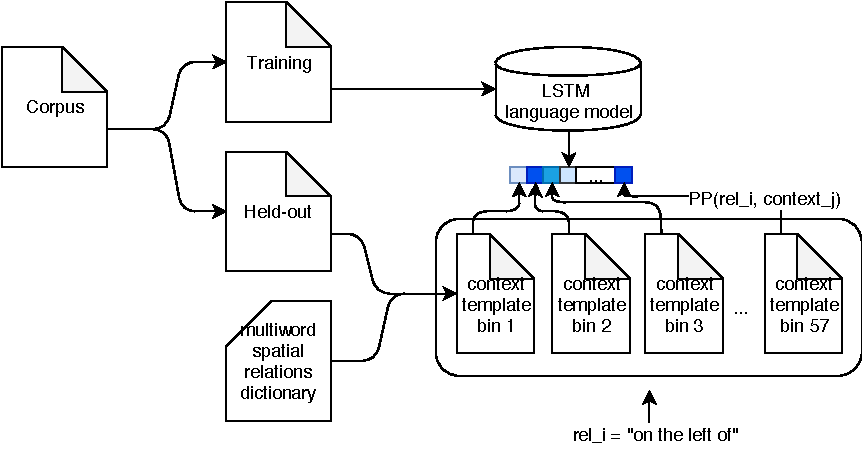
\includegraphics[width=0.75\linewidth]{studies/splu2019/figures/Spatial_Emb_Diagram.pdf}
  \caption{Generating perplexity-based vectors for each spatial relation.}\label{splu2019:fig:diagram}
  \end{center}
\end{figure}

For each of the 67 spatial relations extracted from the larger corpus, there
are 57  collections of sentences (=the number of relations in the smaller
corpus).
Hence, there are
$3,819 (= 67 \times 57)$ possible projections $S_{i \to j}$, where a relation
$i$ is placed in the context $j$, including the case where there is no swapping of relations when $j=i$.  The process is shown in
Figure~\ref{splu2019:fig:diagram}. The vector of resulting perplexities in different
contexts is normalised according to Equation~\ref{splu2019:eq:normal-2} which gives us
perplexity vectors (P-vectors) as shown in Figure~\ref{splu2019:fig:matrix28x26}.

\begin{figure}[ht]
  \begin{center}
  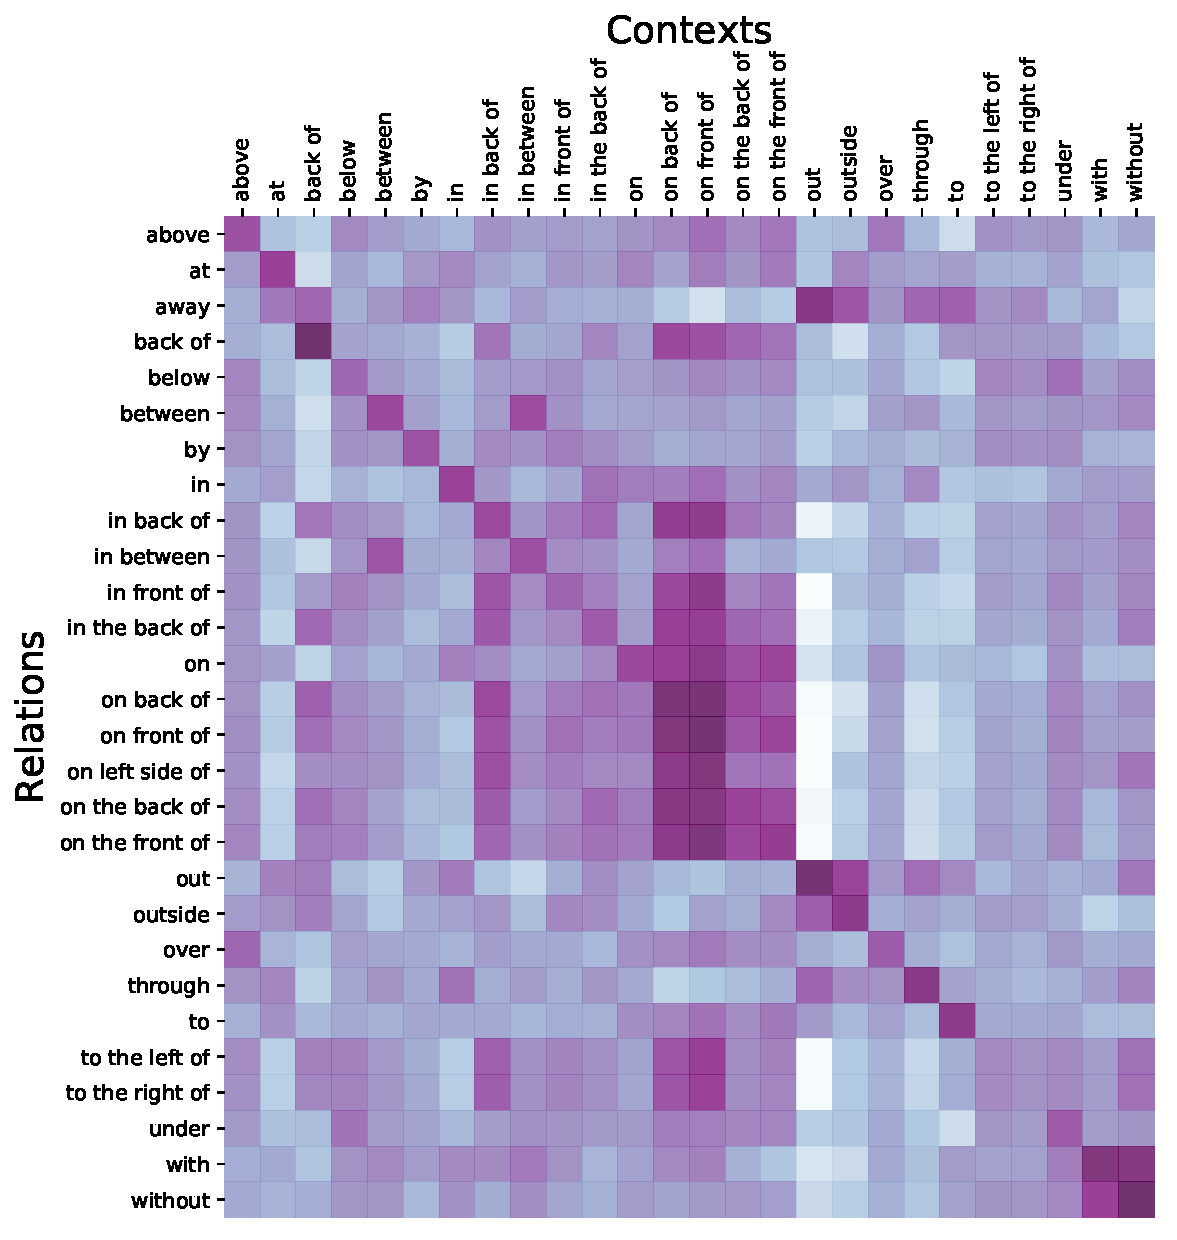
\includegraphics[width=0.75\columnwidth]{studies/splu2019/figures/overall_matrix28x26.pdf}
  \caption{A matrix of perplexity vectors for 28 spatial relations and 26 contexts. For the full $67\times 57$ matrix see %
Appendix~C. The rows represent spatial relations and columns represent the normalised average perplexity of a language model when this relation is swapped in that context.}\label{splu2019:fig:matrix28x26}
  \end{center}
\end{figure}

In addition to the P-vectors we also create representations learned by the word
embedding layer in the generative language model that we train.
For each of the 44 broad single-word spatial relations
we extract a 300-dimensional embedding vector from the pre-trained recurrent
language model (LM-vectors). In order to produce LM-vectors for the multi-word
spatial relations, we %
simply sum the
embeddings of the individual words. For example the embedding vector for ``to
the left of'' is $v_{to} + v_{the} + v_{left} + v_{of}$. The same method is
also used for the GloVe embeddings.


\subsection{Human judgments}\label{splu2019:sec:humanjudgments}
In order to evaluate our word representations we compare them to three sources
of human judgments. The first one are judgments about the the fit of each
spatial relation over different geometric locations of a target object in
relation to a landmark which can be represented as spatial templates
\cite{logan/sadler:1996}. The second are 88,000 word association judgments by English speakers from
\cite{de2018small}. %
In each instance participants were presented a
stimulus word and were asked to provide 3 other words. The dataset contains 4
million responses on 12,000 cues. Based on the collective performance of annotators, the
dataset provides association strengths between words (which contain any kind of
words, not just spatial words) as a measure of their semantic relatedness.
Finally, we collected a new dataset of word similarity judgments using Amazon
Mechanical Turk. Here, the participants were presented with a pair of spatial
relations at a time. Their task was to use a slider bar with a numerical
indicator to express how similar the pair of words are. The experiment is
similar to the one described in \cite{logan/sadler:1996} except that in our
case participants only saw one pair of relations at a time rather than the entire list. The
shared vocabulary between these three datasets covers \emph{left},
\emph{right}, \emph{above}, \emph{over}, \emph{below}, \emph{under},
\emph{near}, \emph{next}, \emph{away}.

\section{Evaluation}\label{splu2019:sec:experiments}


As stated in Section~\ref{splu2019:sec:representations} the P-vectors we have built are
intended to capture the discriminatory power of a generative language model to
encode and discriminate different spatial relations, their functional bias. In
this section we evaluate the P-vectors on several common intrinsic and
extrinsic tests for vectors. If successful, this demonstrates that such
knowledge has indeed been captured by the language model. We evaluate both
single- and multi-word relations.


\subsection{Clustering}
\paragraph{Method} Figure~\ref{splu2019:fig:matrix28x26} and its complete version in %
Appendix~C
show that different spatial relations have
different context fingerprints. To find similar relations in this matrix we can use
\emph{K-means clustering}. %
K-mean is a non-convex problem: different random initialisation may lead to
different local minima.
We apply the clustering on 67 P-vectors for multi-word spatial relations
and qualitatively examine them for various sizes $k$. The optimal number of
clusters is not so relevant here, only that for each $k$ we get reasonable
associations that follow our semantic intuitions.

\paragraph{Results} As shown in Table~\ref{splu2019:tab:clusters}, with $k=30$, the
clustering of perplexity vectors shows acceptable semantics of each cluster.
There are clusters with synonymous terms such as (\ref{item:over}.
\emph{above}, \emph{over}) or (\ref{item:under}. \emph{below}, \emph{under}).
Some clusters have variants of multi-word antonymous such as (\ref{item:topof}.
\emph{on the top of}, \emph{on the bottom of}). Other clusters have a mixture
of such relations, e.g. (\ref{item:leftof}. \emph{right}, \emph{back},
\emph{left}, \emph{side}, and \emph{there}).

\begin{table}
    \begin{tabular}{r|l}
      \begin{minipage}[b]{0.25\linewidth}%
      \begin{footnotesize}
        \begin{enumerate}[noitemsep,topsep=0pt,parsep=0pt,partopsep=0pt]
          \item  to
          \item  on
          \item  away
          \item  here
          \item  into
          \item  from
          \item  during
          \item  back of
          \item  through
          \item  alongside
          \item  along side
          \item  underneath
          \item  in; against
          \item  in front of
          \item \label{item:over} above; over
          \item  to the side
          \item  onto; toward
        \end{enumerate}
      \end{footnotesize}
      \end{minipage}& %
      \begin{minipage}[b]{0.65\linewidth}%
        \begin{footnotesize}
          \begin{enumerate}[noitemsep,topsep=0pt,parsep=0pt,partopsep=0pt]\setcounter{enumi}{17}
            \item  up; down; off
            \item  with; without
            \item  together; out
            \item  outside; inside
            \item  near; beside; by
            \item  top; front; bottom
            \item  in between; between
            \item  along; at; across; around
            \item \label{item:under} beneath; below; under; behind
            \item  \label{item:leftof} right; back; left; side; there
            \item  to the left of; to the right of; next to
            \item  in back of; in the back of; on the back of; at the top of
            \item \label{item:topof} on the top of; on side of; on the bottom of; on left side of; on top of; on the front of; on back of; on the side of; on front of; on bottom of
          \end{enumerate}
        \end{footnotesize}
        \end{minipage}\tabularnewline
    \end{tabular}
	\vspace{0.5em}
    \caption{K-means clusters of spatial relations based on their P-vectors.} %
    \label{splu2019:tab:clusters}
\end{table}

\paragraph{Discussion}  The inspection of the perplexities of two of these
clusters in Figure~\ref{splu2019:fig:clusters} shows that the language model has learned
different selectional properties of spatial relations:
\emph{above} and \emph{over} are generally more selective of their own
contexts, while \emph{to the left of} and \emph{to the right of} show a
higher degree of confusion with a variety of the P-vector contexts.
High degree of confusion in \emph{left} and \emph{right} is consistent with the
observation in \cite{Dobnik:2013aa} that these relations are less dependent on the functional
relation between particular objects and therefore have a higher geometric bias.
On the other hand, \emph{above} and \emph{over} seem to be more selective of
their contexts. The functional distinction between \emph{above} and \emph{over}
is mildly visible: the shades of blue in
\emph{above} are slightly darker than \emph{over}.

\begin{figure}
  \begin{center}
    \begin{minipage}{\linewidth}
      \begin{center}
        \hfill
        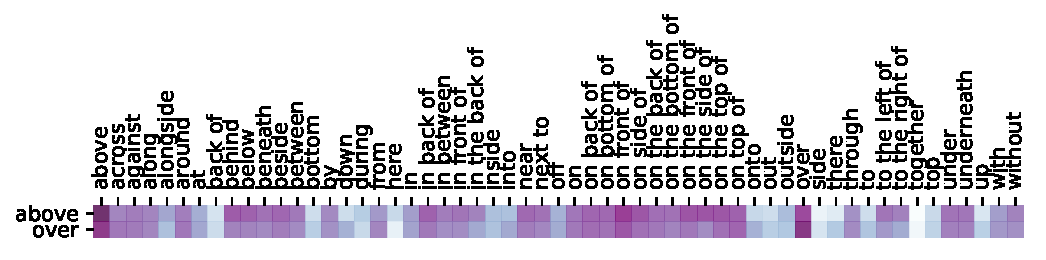
\includegraphics[scale=0.6]{studies/splu2019/figures/above-over.pdf} \\
      \end{center}
    \end{minipage}\\
    \begin{minipage}{\linewidth}
      \begin{center}
        \hfill
        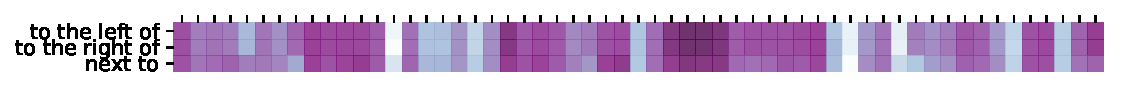
\includegraphics[scale=0.6]{studies/splu2019/figures/left-right.pdf} \\
      \end{center}
    \end{minipage}%
  \caption{The P-vectors of two clusters.
  }
  \label{splu2019:fig:clusters}
\end{center}
\vspace{-5mm}
\end{figure}

\subsection{Analogical reasoning with relations}\label{splu2019:sec:alanogical}
The intrinsic properties of vector representations (the degree to which they
capture functional associations between relations and their objects) can be
tested with their performance in analogical reasoning tasks.
We compare the performance of the P-vectors (Section~\ref{splu2019:sec:contextbins}),
the embeddings of the language model used to create the P-vectors and GloVe
embeddings (Section~\ref{splu2019:sec:training}) in two
analogical tasks which require both geometric and functional reasoning.

\subsubsection{Predicting analogical words}

\paragraph{Method}
The task is similar to the analogy test
\cite{mikolov2013distributed,levy2015improving} where two pairs of words are
compared in terms of some relation ``$a$ is to $a'$ as $b$ is to $b'$".
We manually grouped spatial relations that are opposite in one geometric
dimension to 6 groups.
These are: Group 1: left, right; Group 2: above, below; Group 3: front,
back; Group 4: with, without; Group 5: in, out; and Group 6: up, down.
We generate all possible permutations of these words for the analogical
reasoning task which gives us 120 permutations. We expand these combinations to
include multi-word variants. This dataset has 85,744 possible analogical
questions such as (\emph{above} :: \emph{below}, \emph{to the left of} :: ?).
We accept all variants of a particular relation (e.g.
\emph{to the right side of} and \emph{to the right of}) as the correct answer.




\paragraph{Results} As shown in in Table~\ref{splu2019:tab:analogy}, on the single-word
test suite, the LM-embeddings perform better than other models. On multi-word
test suite the P-vectors perform slightly better. On both test suites, GloVe
trained on Common Crawl performs better than GloVe trained on Visual Genome.
However, its performance on multi-word relations is considerably lower. We
simulated random answers as a baseline to estimate the difficulty of the task.
Although the multi-word test suite has $\sim 700$ times more questions than the
test suite with single-word relations, it is only approximately 2-times more
difficult to predict the correct answer in the multi-word dataset compared to
the single-word dataset.

\begin{table}
    \centering 
      \begin{tabular}{l|r|r}
              & Single word & Multi-words \\
      \hline
      GloVe (CC)   & 0.56 & 0.36 \\
      GloVe (VG)   & 0.43 & 0.29 \\
      \hline
      LM           & 0.86 & 0.45 \\
      P-vectors & 0.62 & 0.47 \\
      \hline
      Random       & 0.11 & 0.05 \\
      \end{tabular}
  	  \vspace{0.5em}
      \caption{The accuracies of different representations on the word analogy test.}
      \label{splu2019:tab:analogy}
      \vspace{-5mm}
\end{table}

\paragraph{Discussion} The perplexity of the language model on complete context
phrases (Multi-words) is as good indicator of semantic relatedness as the word embeddings of
the underlying language model and much better than GloVe embeddings. The good
performance of the P-vectors explains the errors of the language model in
generating spatial descriptions. The confusion between \emph{in front of} and
\emph{on the back of} is similar to the confusion between \emph{to the left of}
and \emph{to the right of} in terms of their distribution over functional
contexts. Hence, a similar lack of strong functional associations allows the
vectors to make inference about geometrically related word-pairs. This
indicates that functional and geometric bias of words are complementary. There
are two possible explanations why P-vectors perform better than LM-embeddings
on multi-word vectors: (i) low-dimensions of P-vectors (57D) intensify the
contribution of spatial contexts for analogical reasoning compared to
high-dimensional LM-embeddings (300D); (ii) summing the vectors of the
LM-embeddings for multi-words reduces their discriminatory effect.

\subsubsection{Odd-one-out}

\paragraph{Method}
Based on the semantic relatedness of words, the goal of this task is to find
the odd member of the three.
The ground truth for this test are the following five categories of spatial
relations, again primarily based on geometric criteria:
X-axis: left, right; Y-axis: above, over, under, below; Z-axis: front, back;
Containment: in, out; and Proximity: near, away.
Only the Y-axis contains words that are geometrically similar but functionally
different, e.g. \emph{above}/\emph{over}.
In total there are 528 possible instances with 3,456 multi-word variations. The
difficulty of the task is the same for both single- and multi-word expressions as the choice is always
between three words. Hence, the random baseline is $0.33$.






\paragraph{Results} Table~\ref{splu2019:tab:oddones} shows the accuracy in predicting
the odd relation out of the three. We also add a comparison to fully geometric
representations captured by spatial templates \cite{logan/sadler:1996}.
\citet{Ghanimifard:2017ab} show that spatial templates can be compared with
Spearman's rank correlation coefficient $\rho_{X,Y}$ and therefore we also
include this similarity measure. Since our groups of relations contain those
that are geometric opposites in each dimension, we take the absolute value of
$|\rho_{X,Y}|$.
Spatial templates are not able to recognise relatedness without the right
distance measure, $|\rho_{X,Y}|$.
LM-embeddings perform better than other vectors in both tests, but P-vectors
follow closely. All models have a low performance on the multi-word test suite.
When using $|\rho_{X,Y}|$
all vectors other than P-vectors produce better results. While we do not have
an explanation for this, it is interesting to observe that $|\rho_{X,Y}|$ is a
better measure of similarity than cosine.


\begin{table}
    \centering 
      \begin{tabular}{r|cc|cc}
        & \multicolumn{2}{c|}{Single word} & \multicolumn{2}{|c}{Multi-words} \\
        & $1-cos$ & $|\rho|$ & $1-cos$ & $|\rho|$ \\
      \hline
      GloVe (CC)   & 0.62 & 0.68 & 0.52 & 0.58 \\
      GloVe (VG)   & 0.61 & 0.61 & 0.58 & 0.59 \\
      \hline
      LM           & 0.87 & 0.90 & 0.82 & 0.88 \\
      P-vectors    & 0.72 & 0.70 & 0.64 & 0.52 \\
      \hline
      Sp Templates & 0.22 & 1.0  &  -   &  -   \\
      \end{tabular}
  \vspace{0.5em}
    \caption{The accuracies in odd-one-out tests.}
    \label{splu2019:tab:oddones}
\end{table}


\paragraph{Discussion} The results demonstrate that using functional
representations based on associations of words
can predict considerable information about geometric distinctions between
relations, e.g. distinguishing \emph{to the right of} and \emph{above}, and
this is also true for P-vectors. As stated earlier, our explanation for this is
that functional and geometric knowledge is in complementary distribution.
This has positive and negative implications for joint vision and language
models used in generating spatial descriptions.
In the absence of geometric information, language models provide strong
discriminative power in terms of functional contexts, but even if geometric
latent information is expressed in them, an image captioning system still needs
to ground each description in the scene geometry.



\subsection{Similarity with human judgments}\label{splu2019:sec:extrinsic}
We compare the cosine similarity between words in LM- and P-vector spaces with
similarities from (i) word association judgments \cite{de2018small},
(ii) our word similarity judgments from AMT, and
(iii) spatial templates (Section~\ref{splu2019:sec:humanjudgments}). We take the maximum
subset of shared vocabulary between them, including \emph{on}, \emph{in} only
shared between (i) and (ii).
Since (i) is an association test, unrelated relations do not have association
strengths. There are 55 total possible pairs of 11 words, while only 28 pairs
are present in (i) as shown in Figure~\ref{splu2019:fig:humansim}.


\begin{figure}
  \begin{center}
    \begin{minipage}{0.4\linewidth}
      \begin{center}
      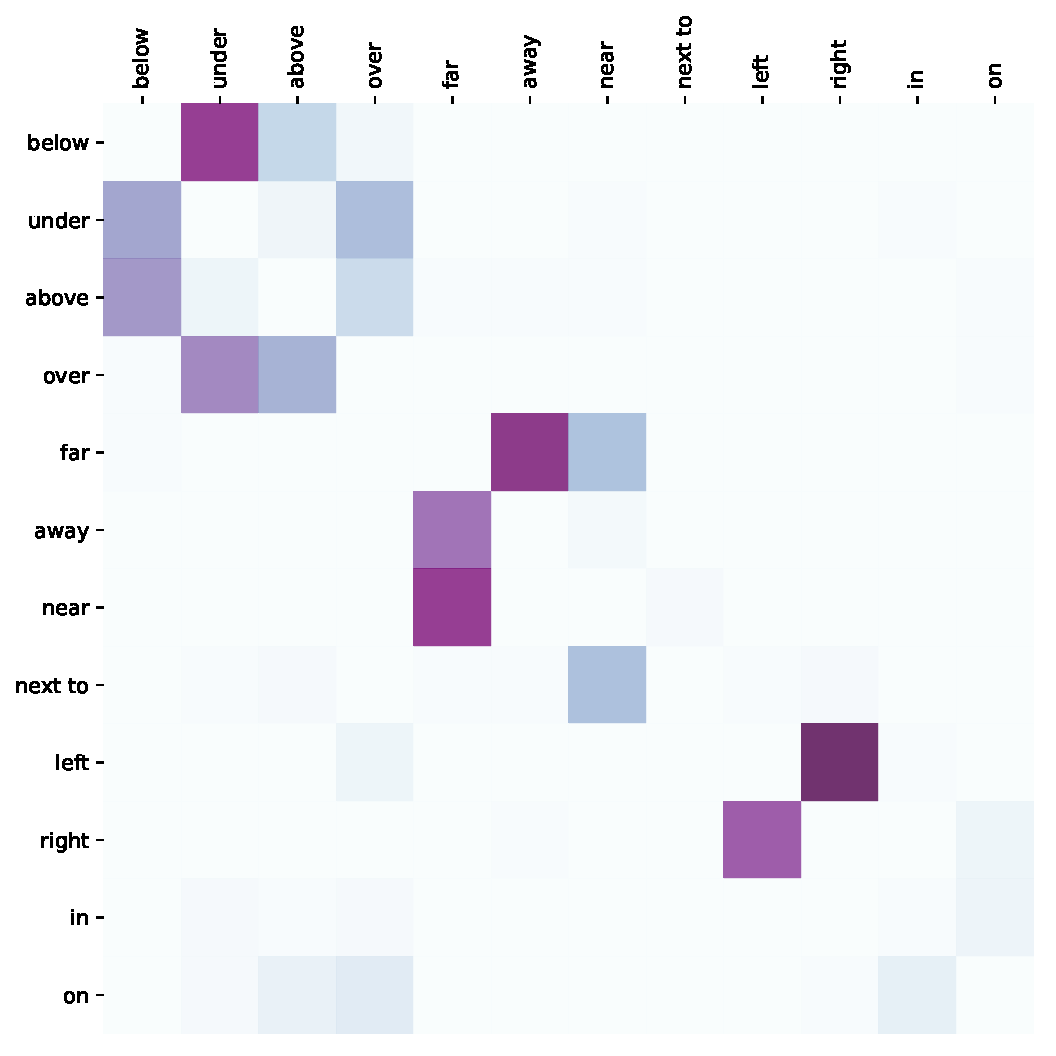
\includegraphics[width=1\columnwidth]{studies/splu2019/figures/word_association_test.pdf} \\
      (a)
      \end{center}%
    \end{minipage}%
    \begin{minipage}{0.4\linewidth}
      \begin{center}
      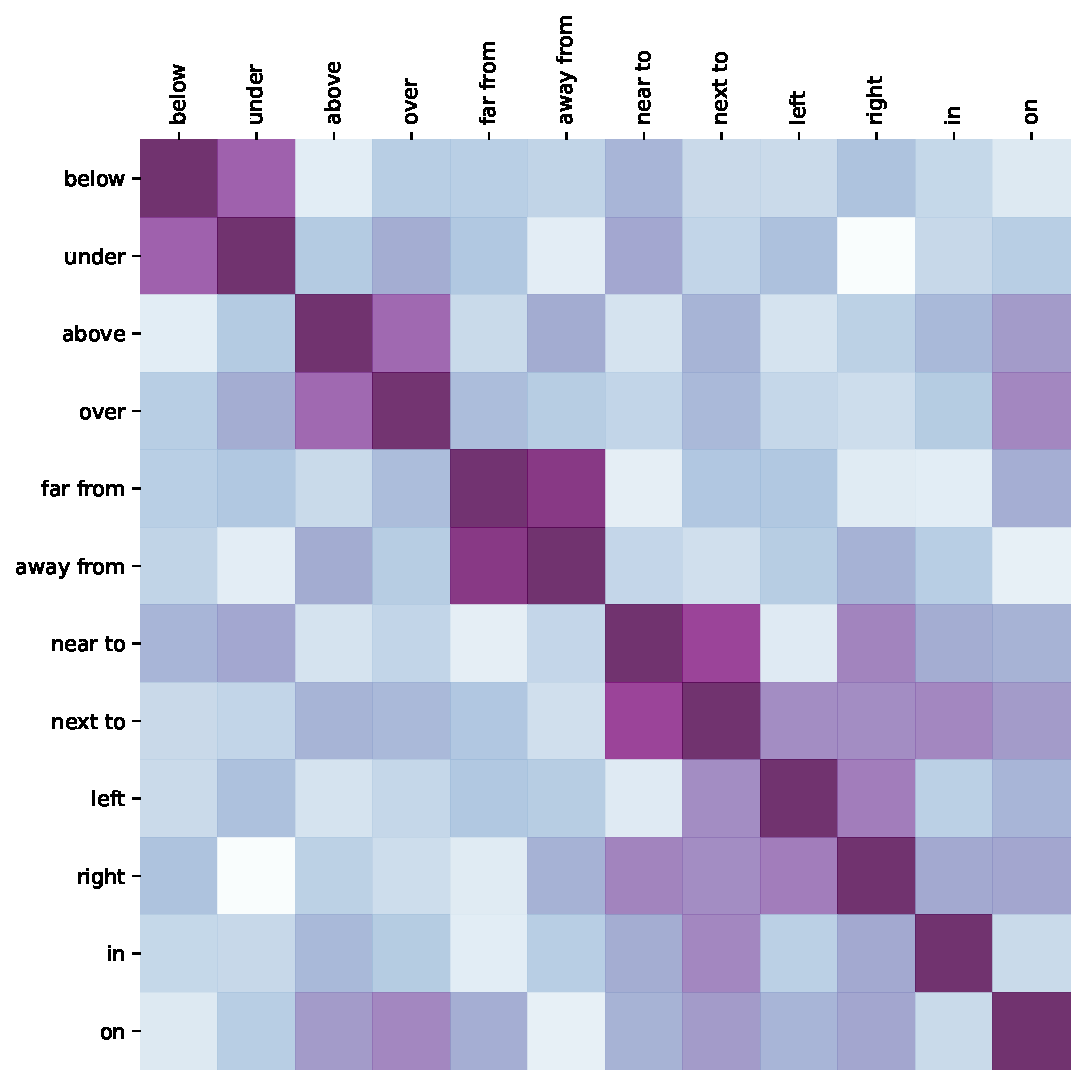
\includegraphics[width=1\columnwidth]{studies/splu2019/figures/relatedness_judgments.pdf} \\
      (b)
      \end{center}%
    \end{minipage}
    \caption{(i) Word association judgments and (ii) word similarity judgments}
  \label{splu2019:fig:humansim}
\end{center}
\end{figure}

\paragraph{Method}
We take the average of the two way association strengths if the association
exists and for (i) %
we assign a zero association for unrelated pairs such as \emph{left} and
\emph{above}. Spearman's rank correlation coefficient $\rho_{X,Y}$ is used to compare the calculated similarities.

\paragraph{Results} Table~\ref{splu2019:tab:humanjudgments} shows ranked
correlations of different similarity measures.
Spatial templates do not correlate with (WA)  word associations and (WS) word
similarities.
On 28 pairs there is a weak negative correlation between spatial templates and
WS. The correlation of similarities of two different human judgments is
positive but weak ($\rho = 0.33$). The similarities predicted by LM-vectors and
P-vectors correlate better with WA than WS.

\begin{table}[ht]
    \centering 
      \begin{tabular}{r|c|c||c|c}
        & \multicolumn{2}{c||}{55 pairs} & \multicolumn{2}{|c}{28 pairs} \\
        \hline
        &
        WA &
        WS &
        WA &
        WS \\
      \hline
      SpTemp & $-0.02$       & $-0.08$ & $0.06$       & $-0.35$ \\
      LM     & $ 0.48^{***}$ & $ 0.15$ & $0.59^{***}$ & $ 0.08$ \\
      P & $ 0.48^{***}$ & $ 0.19$ & $0.40^{**}$  & $-0.08$ \\
      \hline
      \multicolumn{5}{c}{p-values: $* < 0.01$, $** < 0.01$, $*** < 0.001$} \\
      \end{tabular}
	  \vspace{0.5em}
      \caption{
        Spearman's $\rho$ between pairwise lists of similarities.
        WA are similarities based on word associations and WS are direct word
        similarities from human judgments.}
      \label{splu2019:tab:humanjudgments}
\end{table}

\paragraph{Discussion} The low correlation between the two similarities from human judgments
is surprising. Our explanation is that this is because of different priming to
functional and geometric dimension of meaning in the data collection task.
In the WA task participants are not primed with the spatial domain but they are
providing general word associations, %
hence functional associations. On the other hand, in the WS task
participants are presented with two spatial relations, e.g. \emph{left of} and
\emph{right of}, and therefore
the geometric dimension of meaning is more explicitly attended.
We also notice that judgments are not always unison, the same pair may be
judged as similar and dissimilar which further confirms that participants are
selecting between two different dimensions of meaning.
This observation is consistent with our argument that LM-vectors
and P-vectors encode functional knowledge. Both representations correlate
better with WA than with WS.
Finally, \cite{logan/sadler:1996} demonstrate that
WS judgments can be decomposed to dimensions that correlate with the dimensions of the spatial templates. We leave this investigation for our
future work.

\section{Conclusion and future work}\label{splu2019:sec:conclusions}

In the preceding discussion, we have examined what semantic knowledge about spatial relations is captured in
representations of a generative neural language model. In particular, we are
interested if the language model is able to encode a distinction between
functional and geometric bias of spatial relations and how the two dimensions
of meaning interact. The idea is based on earlier work
that demonstrates that this bias can be recovered from the selectivity of
spatial relations for target and landmark objects.
In particular,
(i) we test the difference between multi-word spatial relations at two levels: the
word embeddings which are a form of internal semantic representations in a language model and the
perplexity-based P-vectors which are external semantic representations based on the language model performance;
(ii) we project spatial relations in the contexts of other relations and we
measure the fit of the language model to these contexts using perplexity
(P-vectors);
(iii) we use these contexts to build a distributional model of multi-word
spatial relations;
(iv) in the evaluation on standard semantic similarity tasks, we demonstrate
that these vectors capture fine semantic distinctions between spatial relations;
(v) we also demonstrate that these representations based on word-context associations latently capture geometric knowledge %
that allows analogical reasoning about space; this suggests that functional and geometric components of meaning are complementary: %
(vi) doing so we also demonstrated that generation of
spatial descriptions is also dependent on textual features, even if the system
has no access to the visual features of the scene. This has implications for
baselines for image captioning and how we evaluate visual grounding of
spatial relations.


Our work could be extended in several ways, including by %
(i) using the knowledge about the bias of spatial relations to evaluate captioning
tasks with spatial word substitutions
\cite{shekhar2017vision,shekhar2017foil};
(ii) examining how functional knowledge is complemented with visual knowledge
in language generation \cite{christie2016resolving,delecraz2017correcting}
(iii) using different contextual embeddings such as ELMo \cite{peters2018deep}
and BERT \cite{devlin2018bert}
for the embedding layer of the generative language model rather than our specifically-trained word embeddings; note that P-vectors are representations of collections of context based on the performance of the decoder language model while ELMo and BERT are representations of specific context based on the encoder language model;
(iv) comparing language models for spatial descriptions from different
pragmatic tasks. As the focus of image captioning is to best describe the image
and not for example, spatially locate a particular object, the pragmatic
context of image descriptions is biased towards the functional sense of spatial
relations. Our analysis should be extended
to different kinds of corpora, for example those for visual question answering,
human-robot interaction, and navigation instructions where we expect that precise
geometric locating of objects receives more focus. Therefore, we expect to find a
stronger geometric bias across all descriptions and a lower performance of our representations on analogical
reasoning.

\section*{Acknowledgements}
We are grateful to the anonymous reviewers for their helpful
comments. The research of the authors was supported by a grant from
the Swedish Research Council (VR project 2014-39) to the Centre for
Linguistic Theory and Studies in Probability (CLASP) at Department of
Philosophy, Linguistics and Theory of Science (FLoV), University of
Gothenburg.

\section{Appendix: Perplexity}
\label{splu2019:sec:appendix}
The perplexity in the paper is formulated as follows:
\begin{equation}
PP(S) =  (\prod_{s \in S}{P(w_{1:t}=s)})^{\frac{-1}{|S|}}. \tag{\ref{splu2019:eq:pp}}
\end{equation}
By definition, the perplexity of a model $q$ on a test suit $S$ is defined as follows:
\begin{equation}\label{splu2019:eq:pp_ce}
PP(S) =  2^{H(p,q)}
\end{equation}
\noindent where $H$ is cross entropy, and $p$ is the likelihood of each
possible sample in the test suit. The definition of cross entropy is as follows:
\begin{equation}\label{splu2019:eq:ce}
H(p,q) = - \sum_{x \in S} p(X=x) log_2(q(X=x))
\end{equation}
\noindent where $X$ is a random variable, and $x$ is a possible value of the
random variable. In a forward generative language model, the random variable is
conditioned on the previous words. With test suite being a sequence of words
$S=w_{1:T}$, the likelihood of each word in the sequence is
$p(w_t)=\frac{1}{T}$, and the cross entropy of the model on the samples is:
\begin{align}\label{splu2019:eq:ce_lm}
H(p, q) &= - \sum_{t = 1}^{T}{p(w_t) log_2(q(w_t|w_{1:t-1}))} \\
&= -  \frac{1}{T} \sum_{t = 1}^{T}{log_2(q(w_t|w_{1:t-1}))}
\end{align}
\noindent where $w_t$ is a token at a time $t$, in a sequence with maximum $T$
tokens, $w_{1:t} = w_1, w_2, ..., w_t$.  Therefore the perplexity is:
\begin{align}
PP(S) &= 2^{- \frac{1}{T} \sum_{t = 1}^{T}{log_2(q(w_t|w_{1:t-1}))}}\label{splu2019:eq:pp_ce1} \\
&= (\prod_{t = 1}^{T}{q(w_t|w_{1:t-1})})^{- \frac{1}{T}}\label{splu2019:eq:pp_ce2}
\end{align}
\noindent Equation~\ref{splu2019:eq:pp_ce2} is often used as definition of perplexity in
language models \cite{goodman2001bit} and Equation~\ref{splu2019:eq:pp_ce1} is its
numeric computation to avoid underflow due to adding logits. \\
There are two ways to extend the definition to the case when perplexity is
calculated for a collection of sentences. (i) We can treat the corpus as a long
sequence of tokens and use the previous equations. (ii) We can use
Equation~\ref{splu2019:eq:ce} with a change to the model definition, from a token model
to a sentence model. The benefit of this method is that it assigns the same
likelihood for each sentence regardless of its length. In this case, the chain
rule is used for the sentence model. The likelihood of each sentence is one
over the number of sentences in the test suite, $p(s)=\frac{1}{|S|}$:
\begin{align}\label{splu2019:eq:ce_lm2}
H(p, q) &= - \sum_{s \in S}{p(s) log_2(\hat{P}(s))} \\
&= - \frac{1}{|S|} \sum_{s \in S}{log_2(\hat{P}(s))}
\end{align}
Based on the chain rule, the sentence model can be calculated as follows:
\begin{align}\label{splu2019:eq:lm2}
\hat{P}(w_{1:T}=s) &= \prod_{t = 1}^{T}{q(w_t|w_{1:t-1})} \\ \label{splu2019:eq:lm2logits}
log_2(\hat{P}(w_{1:T}=s)) &= \sum_{t = 1}^{T}{log_2(q(w_t|w_{1:t-1}))}
\end{align}
Perplexity in this case is defined as in Equation~\ref{splu2019:eq:pp} here repeated as
Equation\ref{splu2019:eq:pp2}:
\begin{equation}\label{splu2019:eq:pp2}
PP(S) =  (\prod_{s \in S}{\hat{P}(w_{1:T_s}=s)})^{\frac{-1}{|S|}}
\end{equation}
\noindent which instead of using the product is computed as a sum of
logits from Equation~\ref{splu2019:eq:ce_lm2} and \ref{splu2019:eq:lm2logits}.


\section{Appendix: Examples of images from Visual Genome}\label{splu2019:sec:appendix-image}
Figure~\ref{splu2019:fig:examples1} and Figure~\ref{splu2019:fig:examples2} are the examples from VisualGenome which their region descriptions are used in the paper as examples of relation-context substitution table. 
\begin{figure*}[h!]
	\centering
	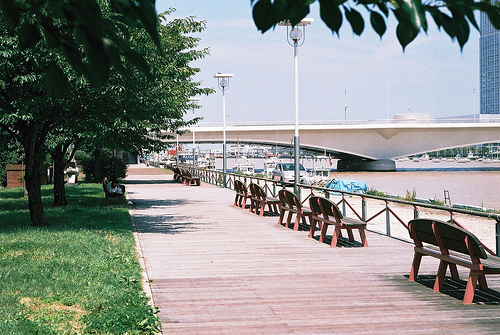
\includegraphics[width=0.65\linewidth]{studies/splu2019/figures/2367586.jpg}
	\caption{
		image\_id = 2367586 \\
		tall building above the bridge \\
		bench below the green trees \\
		car next to the water}\label{splu2019:fig:examples1}
\end{figure*}

\begin{figure*}[h!]
	\centering
	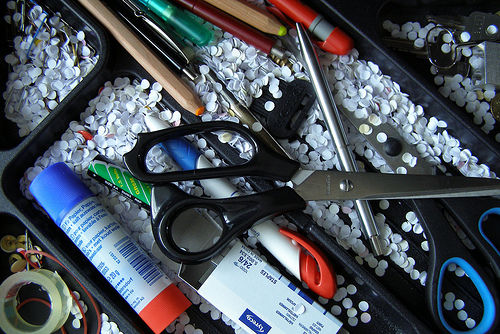
\includegraphics[width=0.65\linewidth]{studies/splu2019/figures/2320485.jpg}
	\caption{
		image\_id = 2320485 \\
		scissors above the pen \\
		the pen is below scissors \\
		a ball-pen next to the scissorts}\label{splu2019:fig:examples2}%
\end{figure*}

\pagebreak
\section{Appendix: Complete P-vectors}\label{splu2019:sec:appendix_plots}
Figure~\ref{splu2019:fig:matrix} is the full presentation of P-vectors.
\begin{figure*}[h!]
	\begin{center}
		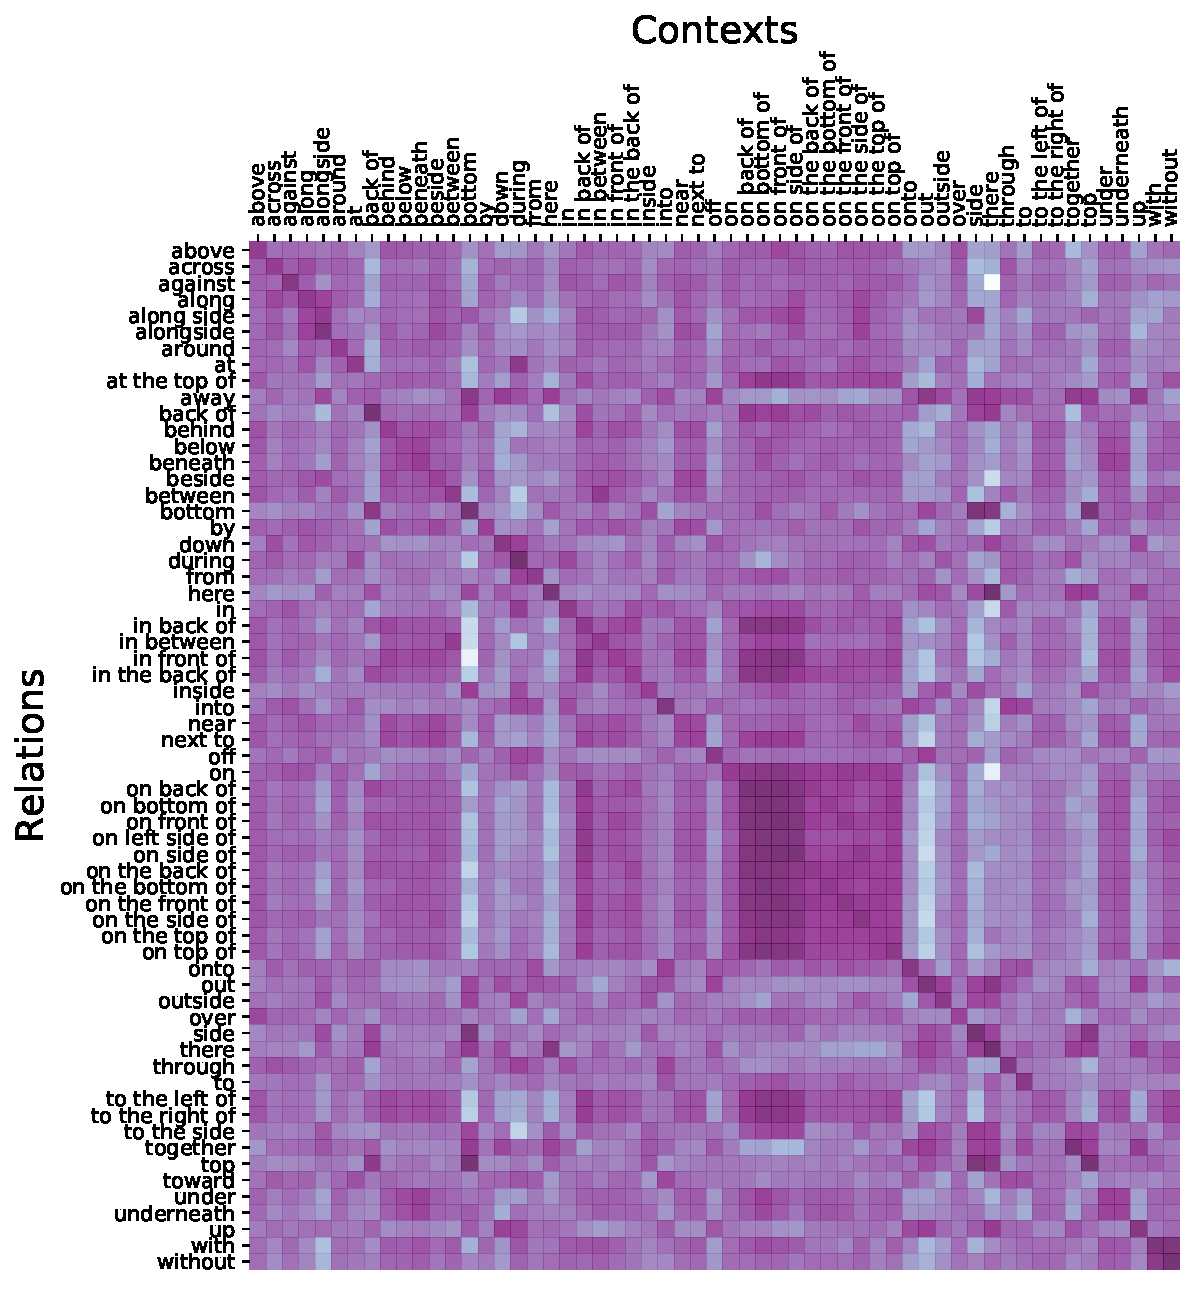
\includegraphics[width=0.9\linewidth]{studies/splu2019/figures/overall_matrix57x63.pdf}
		\caption{Perplexity vectors for 67 spatial relations on 57 context bins.}
		\label{splu2019:fig:matrix}
	\end{center}
\end{figure*}

\section{Appendix: Similarity Judgment Dataset}\label{splu2019:sec:similarity_dataset}
In total 66 worker in Amazon Mechanical Turk annotated the word similarity. For each word pair, we collected 10 judgments. The word pairs vertically in random order were presented to annotators to judge their similarity. The input form was a slider in the web interface which they could freely adjust the indicator position between dissimilar and similar rating (Figure~\ref{splu2019:fig:screenshot}). In order to identify the bad annotators, we randomly asked the annotators to judge similarity between ``\emph{green}" and one of the spatial relations, we also asked similarity judgment between a spatial relation and itself. If the answer to similarity with green was higher than \%60, or the answer for self similarity was lower than \%90, all contributions of that worker were taken out from the dataset. This cleaning technique removed 9 workers in total, which left us about 7 annotation on each word pair.

\begin{figure}[h!]
	\begin{center}
		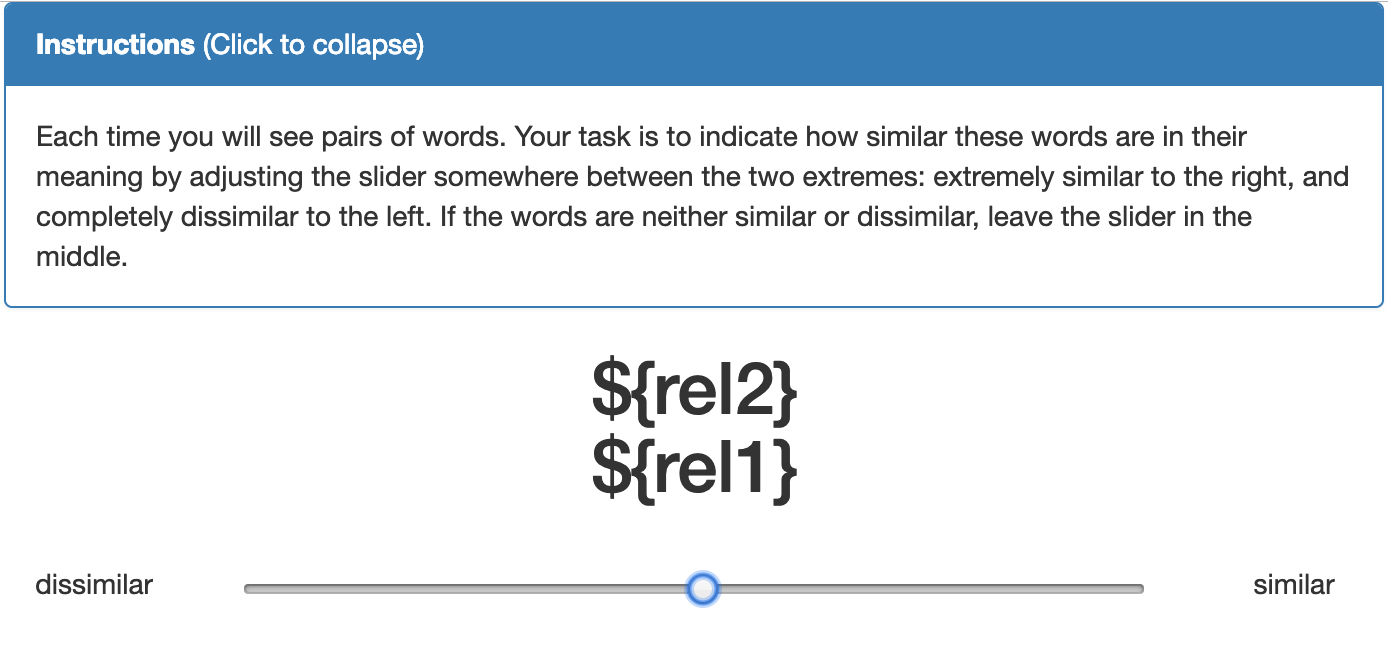
\includegraphics[width=0.85\linewidth]{studies/splu2019/figures/amt_layout_screenshot.png}
		\caption{The layout which presents the similarity judgment question.}
		\label{splu2019:fig:screenshot}
	\end{center}
\end{figure}

\clearpage
\bibliographystyle{acl_natbib}
\bibliography{studies/splu2019/references.bib}

